\documentclass[conference,compsoc]{IEEEtran}
\usepackage{datetime}
\usepackage{caption}
\usepackage{listings}
\usepackage{cite} 
\usepackage{hyperref}
\usepackage{xcolor}
\usepackage{pgfplots}
\usepackage{graphicx}
\usepackage{float}

\usepgfplotslibrary{polar}
\pgfplotsset{compat=1.17} 
\usetikzlibrary{shapes.geometric, arrows}

\tikzstyle{startstop} = [rectangle, rounded corners, minimum width=3cm, minimum height=1cm, text centered, draw=black, fill=red!30]
\tikzstyle{io} = [trapezium, trapezium left angle=70, trapezium right angle=110, minimum width=3cm, minimum height=1cm, text centered, draw=black, fill=blue!30]
\tikzstyle{process} = [rectangle, minimum width=3cm, minimum height=1cm, text centered, draw=black, fill=orange!30]
\tikzstyle{arrow} = [thick,->,>=stealth]

\begin{document}

% paper title
\title{GreenIT Article Review Report on\\
"How realistic are claims about the benefits of using digital technologies for GHG emissions mitigation?"
\\

%current time
{\small \today~-~\currenttime}}

% student name
\author{\IEEEauthorblockN{TITCHEU YAMDJEU Pierre Wilfried}
	\IEEEauthorblockA{University of Luxembourg\\
		Email: pierre.titcheu.001@student.uni.lu}
	\\
	($\pm$ 5 pages)\\}

% make the title area
\maketitle

% abstract
\begin{abstract}

	This report conducts a critical review of "How realistic are claims about the benefits of using digital technologies for GHG emissions mitigation?" by Aina Rasoldier et al. The paper delves into the validity of claims surrounding digital technologies, particularly focusing on carpooling platforms, in their role of reducing greenhouse gas (GHG) emissions. It not only questions the prevailing assumptions but also proposes a set of guidelines for a more grounded and realistic assessment of these digital solutions in the context of environmental sustainability.

\end{abstract}

% Context
\section{Introduction ($\pm 0,5p$)}

In their insightful paper, Aina Rasoldier et al.
critically assess the potential of digital technologies
in mitigating greenhouse gas (GHG) emissions, with a special focus on carpooling platforms. Amidst the growing digitalization of various sectors and its associated environmental impacts, the paper examines the prevalent belief that digital solutions can significantly contribute to GHG emission reduction. This research is pivotal as it intersects with the domain of GreenIT, which emphasizes leveraging technology to tackle environmental challenges. The authors delve into the real-world implications of digital technologies on environmental sustainability, highlighting the necessity for comprehensive assessments that extend beyond mere technological advancements. By scrutinizing the methodological approaches in current studies, this paper identifies significant gaps and proposes a set of guidelines to ensure more accurate evaluations. It underscores the importance of contextualizing these technologies within broader global strategies for GHG emission reduction, thereby contributing a nuanced perspective to the discourse on the role of digital solutions in climate change mitigation.

% Research Problem 
\section{Research problem addressed ($\pm 0,5p$)}

The paper addresses the research problem of evaluating
the actual impact of digital technologies on GHG emissions.
It questions the prevailing optimistic claims regarding the
efficacy of digital solutions, specifically carpooling platforms,
in environmental conservation. The research objectives include
establishing a framework for a more realistic and comprehen-
sive assessment of digital solutions in GHG mitigation. The
paper hypothesizes that current evaluations of digital tech-
nologies for GHG reduction are often overestimated, lacking
in critical analysis of life-cycle impacts, structural impacts,
and rebound effects. It aims to substantiate this hypothesis
by applying its proposed evaluation framework to the case of
carpooling platforms.

% Paper references review 

\section{Extended Literature Review (±1p)}

The paper "How realistic are claims about the benefits of using digital technologies for GHG emissions mitigation?" by Aina Rasoldier et al. offers a nuanced critique of the existing literature at the intersection of digital technology and GHG emissions mitigation. The review situates the discussion within a historical context of environmental awareness and action, referencing pivotal moments like the United Nations Stockholm Conference on the Human Environment (1972) and the subsequent formation of the UNEP, charting the evolution of global environmental consciousness.

The Brundtland Report (1987) is significant for introducing the enduring concept of sustainable development, a key theme underlying the paper's focus. This concept, emphasizing the balance between current needs and future sustainability, is crucial in assessing the long-term viability of digital technologies.

The United Nations Sustainable Development Goals (SDGs), particularly SDG 13 - Climate Action, provide a comprehensive framework for evaluating the alignment of digital solutions with global environmental objectives. This backdrop is essential for understanding the paper’s scrutiny of digital innovations in the context of climate action.

The methodology of Life Cycle Assessment (LCA), as outlined by ISO 14040 and ISO 14044, is a critical tool referenced in the paper. LCA enables an all-encompassing evaluation of the environmental impact of technologies throughout their entire lifecycle. This approach is integral to understanding the complete environmental implications of digital solutions.

The European Green Deal, aiming for climate neutrality by 2050, reflects the policy context influencing the development and adoption of digital technologies. The integration of digital strategies within environmental policies, as advocated by the Green Deal, resonates with the paper's examination of digital approaches to GHG mitigation.

The paper delves into the distinction between Green IT and IT for Green, elucidating the dual role of digital technologies in environmental sustainability. While Green IT focuses on making IT infrastructure sustainable, IT for Green highlights the application of IT in enhancing broader environmental sustainability.

A substantial portion of the literature review is devoted to critiquing the methods used in existing studies for evaluating digital solutions' environmental benefits. The paper underscores the necessity for detailed, context-specific assessments and cautions against the overestimation of the benefits of digital solutions. It emphasizes the integration of these technologies into realistic and comprehensive strategies for GHG reduction, challenging the simplistic narratives often presented in the literature.

% Contributions 
\section{Scientific contributions w.r.t. GreenIT and IT for Green ($\pm 2p$)}

\subsection{Introduction to the Interplay between GreenIT and IT for Green}

The paper by Rasoldier et al. delves deeply into the intertwined roles of Green Information Technology (GreenIT) and Information Technology for Green (IT for Green) in advancing environmental sustainability. It emphasizes how IT, traditionally seen as a contributor to ecological problems, also holds significant potential for environmental conservation and GHG emissions reduction. By exploring various digital solutions, including carpooling platforms, the study illuminates the complex yet pivotal role of technology in both exacerbating and alleviating environmental challenges. This section could benefit from a focus on the paper's critical analysis of common misconceptions and overestimations regarding the environmental benefits of digital technologies. It also stresses the importance of adopting a balanced and realistic approach in assessing the environmental impacts of such technologies.

\subsection{Detailed Examination of GreenIT}

\subsubsection{Life Cycle Assessment and Sustainability of ICT}

The paper presents a critical analysis of the Life Cycle Assessment (LCA) of ICT, adhering to ISO standards 14040 and 14044. It emphasizes the holistic environmental impact of ICT, from production to disposal. The focus on life-cycle impacts underlines the significance of direct effects of ICT services. By incorporating multi-criteria assessment methods, the paper broadens the scope of evaluating environmental impacts, including GHG emissions, resource consumption, and waste generation, aligning with global sustainability goals.

\subsubsection{Green Standards and Metrics in ICT}

The research further elucidates the importance of robust methodologies in measuring ICT's environmental impacts. It delves into the critical analysis of GHG emissions and energy use, core metrics for GreenIT sustainability. This approach aligns with the main metrics discussed for GreenIT, such as primary energy consumption and greenhouse gas emissions. The detailed examination of these metrics in the paper enhances our understanding of the environmental footprint of digital technologies, pivotal for the development of sustainable IT systems.

\subsection{Contributions to IT for Green}

\subsubsection{Digital Solutions in Mitigating GHG Emissions}

In the realm of IT for Green, the paper explores how digital technologies can aid in achieving environmental sustainability goals, particularly in the context of SDG 13 - Climate Action. It evaluates the potential of digital solutions in reducing GHG emissions across various domains, including transportation, energy, and agriculture. This evaluation is in line with the  focus on leveraging IT to support specific Sustainable Development Goals (SDGs).

\subsubsection{Balancing GreenIT and IT for Green}

The paper addresses the balance between the environmental costs of developing and using digital technologies (GreenIT) and their benefits for environmental sustainability (IT for Green). This perspective acknowledges the complex relationship between IT and environmental goals, as discussed in the lecture on GreenIT and IT for Green interplay.

In section 4.2, the paper details the scenarization process for evaluating GHG emissions in the mobility sector, focusing on carpooling platforms. It contrasts scenarios with and without platform-enabled carpooling to assess avoided emissions. The paper also highlights the challenges in quantifying the emissions of digital infrastructure due to lack of data and varying platform types. This nuanced approach underscores the complexity of accurately measuring the environmental impact of digital solutions and the importance of comprehensive scenario analysis in sustainability assessments.

\subsection{Evaluation of Digital Technologies' Impact on GHG Mitigation}

\subsubsection{Critical Analysis of Claimed Benefits}

The paper critically examines the often-stated benefits of digital technologies in mitigating greenhouse gas (GHG) emissions. It probes the validity of these claims by exploring various scenarios and hypotheses underlying these assessments. This aligns with the  emphasis on the importance of a rigorous and transparent evaluation process in GreenIT, where claimed benefits must be substantiated with credible and verifiable data.

\subsubsection{Methodological Rigor in Assessments}

In line with the  focus on methodological rigor, the paper proposes guidelines for studies evaluating the impact of digital solutions on GHG emissions. These guidelines include:
\begin{enumerate}
	\item \textbf{Life-Cycle Analysis (LCA)}: Emphasizes the importance of using LCA, as per ISO standards 14040 and 14044, to assess the full environmental impact of digital technologies from production to disposal.
	\item \textbf{Structural Effects}: Addresses the need to consider broader impacts, including second-order effects and structural changes in systems and processes.
	\item \textbf{Scenarization}: Advocates for creating multiple scenarios to predict and assess the potential impacts of digital solutions on GHG emissions accurately.
	\item \textbf{Global Sustainability Objectives}: Stresses the importance of aligning digital solutions with broader environmental goals and sustainability objectives.
\end{enumerate}
These guidelines stress the importance of life-cycle analysis, consideration of structural impacts, and the connection of proposed solutions with global sustainability goals. This approach is crucial for ensuring that the evaluations of digital technologies' contributions to GHG reduction are comprehensive and grounded in reality.

\subsection{Implications for Policy and Strategy}

\subsubsection{Influence on Regulations and Policies}

The paper's findings have implications for the regulation of the ICT sector and the development of digital strategies aimed at environmental sustainability. By providing a clear assessment of the environmental impacts of digital technologies, the paper supports the  discussion on the need for informed policy-making in GreenIT and IT for Green. This is particularly relevant in the context of the European Union's Green Deal and the UN's Sustainable Development Goals, which prioritize sustainability in technology development and use.

\subsubsection{Identifying Research Gaps and Future Directions}

The paper highlights key research gaps in the field of GreenIT and IT for Green, emphasizing the need for ongoing exploration and innovation. It identifies specific areas where current research is lacking, such as the comprehensive assessment of the environmental impact of ICT through Life Cycle Assessment, understanding the structural and second-order effects of digital solutions, and the development of more accurate scenarization methodologies. These identified gaps pave the way for future research to deepen our understanding of the relationship between ICT and environmental sustainability, and to develop more effective strategies for leveraging technology in achieving sustainability goals.

\subsection{Real-world Applications and Case Studies}

\subsubsection{Practical Insights into GreenIT Strategies}

The paper provides practical insights into how digital technologies can be implemented in real-world scenarios to achieve environmental benefits. This practical approach resonates with the  focus on applying GreenIT strategies in diverse contexts, such as energy-efficient computing and sustainable data centers.

\subsubsection{Case Study Analysis}

By examining specific case studies, such as the role of digital platforms in carpooling and its impact on GHG emissions, the paper offers concrete examples of how IT can contribute to environmental sustainability. These case studies illustrate the  emphasis on the practical application of GreenIT and IT for Green principles in addressing real-world challenges.

\subsection{Sustainable Development Goals (SDGs) and Digital Solutions}

\subsubsection{Alignment with SDGs}

The paper's analysis of digital technologies in GHG mitigation aligns with several Sustainable Development Goals (SDGs), particularly SDG 13 (Climate Action). This connection underscores the  focus on how IT solutions can support broader sustainability objectives. The research emphasizes the potential of digital technologies to contribute to these global goals, reinforcing the concept of IT for Green.

\subsubsection{Contributions to Specific SDGs}

Beyond GHG mitigation, the paper's implications extend to other SDGs, such as SDG 7 (Affordable and Clean Energy) and SDG 11 (Sustainable Cities and Communities). By evaluating digital solutions in transportation and energy sectors, the research contributes to understanding how GreenIT can aid in achieving multiple sustainability targets.

\subsection{GreenIT and Environmental Assessment}

\subsubsection{Life Cycle Assessment (LCA) in Evaluations}

Consistent with the  emphasis on holistic assessments, the paper advocates for the use of Life Cycle Assessment (LCA) in evaluating digital solutions. This approach ensures that all environmental impacts of digital technologies, from production to disposal, are considered, thereby promoting a comprehensive understanding of their environmental footprint.

\subsubsection{Multi-Criteria Assessment Methods}

The paper's methodology resonates with the  discussion on multi-criteria assessment methods in GreenIT. By considering various environmental impacts, including GHG emissions, resource use, and energy consumption, the research aligns with the broader perspective of environmental sustainability in IT.

\subsection{Implications for GreenIT and IT for Green}

\subsubsection{Balancing IT Development and Environmental Impact}

The paper's findings highlight the delicate balance between advancing digital technologies and managing their environmental impacts. This aligns with the  theme of finding sustainable pathways for IT development, ensuring that technological progress does not come at the expense of environmental degradation.

\subsubsection{Guiding Future Research and Development}

The research offers crucial insights for future studies in GreenIT and IT for Green, particularly in addressing current limitations and proposing development paths. It underscores the modest contribution of digital solutions like carpooling platforms to GHG mitigation and the need for more effective strategies. Future research should focus on overcoming obstacles to widespread adoption of such technologies and minimizing negative structural effects. Additionally, there is a significant research gap in understanding the specific impacts of digital platforms on global GHG mitigation scenarios, as well as in identifying and tackling the barriers to their effectiveness. The paper calls for a systematic review of strategies to enhance carpooling and other digital solutions, considering behavioral and logistical challenges, to meaningfully contribute to climate change mitigation.

% Analysis and discussion 
\section{Critical Analysis ($\pm 1p$)}

\subsection{Analysis of Paper's Contributions}

\subsubsection{Contribution to GreenIT and IT for Green}

The publication's exploration into the realistic benefits of digital technologies for GHG emissions mitigation is a vital contribution to both GreenIT and IT for Green concepts. While GreenIT primarily focuses on minimizing the environmental impact of IT itself, IT for Green emphasizes using IT to improve environmental sustainability across various sectors. The paper bridges these two areas by assessing the efficacy of digital solutions in reducing GHG emissions, thereby contributing to broader environmental goals.

\subsubsection{Applicability to Real-World Scenarios}

The research's real-world applicability is commendable. It goes beyond theoretical discussions to evaluate actual digital technologies and their potential in real-world scenarios. This practical approach aligns well with the  emphasis on applying theoretical knowledge to real-world challenges in sustainability.

\subsection{Related Work and Its Contextualization}

\subsubsection{Comprehensive Review of Existing Literature}

The paper does an excellent job of reviewing existing literature and contextualizing its research within the broader field of environmental sustainability in IT. This extensive review not only helps in understanding the current state of research but also in identifying gaps that the paper aims to address.

\subsubsection{Integration of Multi-Disciplinary Perspectives}

The inclusion of multi-disciplinary perspectives, particularly the intersection of technology, environmental science, and policy, is a strong point of the paper. This approach reflects the  focus on the interdisciplinary nature of sustainability issues, where solutions often require input from various fields.

\subsection{Limitations and Areas for Improvement}

\subsubsection{Scope of Technology Assessment}

One limitation of the paper is its scope in assessing the impact of digital technologies. While it does provide valuable insights, the focus is somewhat narrow, primarily centered around GHG emissions. As discussed in the lecture, a more holistic approach, considering other environmental aspects like resource depletion, e-waste, and ecological impacts, would provide a more comprehensive understanding of the sustainability of digital technologies.

\subsubsection{Potential for Broader Impact Analysis}

The paper could benefit from a broader analysis of the indirect impacts of digital solutions, such as societal and economic effects. This aspect aligns with the  emphasis on considering all dimensions of sustainability, not just environmental, to truly assess the impact of technology on sustainable development.

\subsection{Future Work Suggestions}

\subsubsection{Expanding the Methodological Framework}

The future work suggested by the paper, including refining and expanding its methodological framework, is crucial. Applying its guidelines to a wider range of digital solutions would validate and potentially improve their utility in diverse contexts. This suggestion resonates with the  call for continuous improvement and adaptation in sustainability research.

\subsubsection{Long-Term Impact Studies}

Another area for future research is long-term impact studies of digital technologies on sustainability. Understanding the long-term effects, both positive and negative, will be essential in aligning IT developments with sustainable development goals, as highlighted in the lecture.

\subsection{Deeper Examination of Environmental Impacts}

\subsubsection{Comprehensiveness in Environmental Impact Analysis}

While the paper's focus on GHG emissions is pertinent, a more comprehensive analysis encompassing a broader range of environmental impacts would be beneficial. This could include factors like water usage, land use changes, and biodiversity impacts. Such an expanded scope would align with the  emphasis on a holistic approach to environmental sustainability in IT.

\subsubsection{Integration of Life Cycle Assessment (LCA)}

Incorporating Life Cycle Assessment (LCA) methodologies could enhance the depth of the paper's analysis. LCA would provide a more nuanced understanding of the environmental impacts of digital technologies throughout their lifecycle, from production to disposal, resonating with the  discussion on the importance of considering the entire lifecycle in sustainability assessments.

\subsection{Socio-Economic Considerations and Sustainability}

\subsubsection{Balancing Technology and Human Factors}

The paper could further explore the balance between technological advances and socio-economic factors. Understanding how digital technologies interact with human behaviors, economic systems, and societal structures is crucial for effective GHG mitigation strategies, as highlighted in the lecture series.

\subsubsection{Addressing Equity and Accessibility}

Future work should also consider the equity and accessibility aspects of digital solutions for GHG mitigation. Ensuring that these technologies are accessible and beneficial across different socio-economic groups aligns with the comprehensive view of sustainability discussed in the lecture, where social equity is a key pillar.

\subsection{Policy Implications and Recommendations}

\subsubsection{Engagement with Policy and Regulatory Frameworks}

The paper's findings have significant policy implications. Future research could focus on translating these findings into actionable policy recommendations, thus bridging the gap between research and policy-making, a topic emphasized in the lecture series.

\subsubsection{Collaboration with Stakeholders}

Collaborating with a range of stakeholders, including government bodies, industry players, and civil society, can enhance the impact of the research. Such collaboration aligns with the  focus on multi-stakeholder engagement as a critical component of sustainable development.

\subsection{Technological Innovation and Sustainable Development}

\subsubsection{Exploring Emerging Technologies}

The exploration of emerging technologies and their potential role in GHG mitigation is an area ripe for future research. Investigating innovative technologies aligns with the  emphasis on leveraging technological advancements for sustainable development.

\subsubsection{Consideration of Technological Limitations and Risks}

It's also crucial to critically assess the limitations and potential risks associated with deploying new technologies for environmental sustainability, as discussed in the lecture. This includes understanding the trade-offs and unintended consequences that might arise.

\subsection{Conclusion}

The publication provides a valuable contribution to the field of environmental sustainability in IT, aligning well with the concepts discussed in the lecture series. However, expanding its scope to include a more comprehensive environmental impact analysis, considering socio-economic factors, and engaging more deeply with policy implications would enhance its relevance and applicability.

\subsection{Future Research Directions}

\subsubsection{Advancing Methodological Rigor}

Future research based on this paper's findings should aim for greater methodological rigor, especially in scenario modeling and impact assessment. Incorporating robust, diverse, and realistic scenarios, as emphasized in the lecture, can lead to more accurate and meaningful insights into the role of digital technologies in GHG mitigation.

\subsubsection{Interdisciplinary Approaches}

The paper highlights the need for interdisciplinary research combining IT, environmental science, economics, and social sciences. Such an approach resonates with the  emphasis on cross-disciplinary collaboration for comprehensive sustainability solutions.

\subsection{Limitations of the Study}

\subsubsection{Scope of the Research}

While the paper's focus on digital solutions for GHG mitigation is timely, its narrow focus on certain aspects of environmental impacts limits its applicability. Future studies should expand the scope to include a wider range of environmental and social impacts, in line with the  broader perspective on sustainability.

\subsubsection{Data and Methodological Constraints}

The reliance on specific datasets and methodologies may limit the generalizability of the paper's findings. Future work should explore diverse data sources and methodologies, as suggested in the lecture, to enhance the robustness and applicability of the research.

\subsection{Practical Implications}

\subsubsection{Implementing Sustainable IT Practices}

The paper's findings have practical implications for implementing sustainable IT practices in various sectors. This aligns with the  discussion on the practical application of sustainability principles in the IT industry.

\subsubsection{Guidance for Practitioners and Policymakers}

The research provides valuable insights for practitioners and policymakers. Future work should focus on translating these insights into actionable strategies and policies, as underscored in the lecture, to effectively harness digital technologies for environmental sustainability.

\subsection{Conclusion}

Overall, the paper makes a significant contribution to understanding the role of digital technologies in GHG emissions mitigation. However, by addressing its limitations and incorporating the  comprehensive approach to sustainability, future research can provide more nuanced and actionable insights. This will be crucial in leveraging IT for environmental sustainability and achieving broader sustainable development goals.

\section*{References}

\begin{enumerate}
	\item Rasoldier, A., Combaz, J., Girault, A., Marquet, K., \& Quinton, S. (2022). How realistic are claims about the benefits of using digital technologies for GHG emissions mitigation? In LIMITS '22: Workshop on Computing within Limits, June 21–22, 2022.
	\item Brundtland, G. H. (1987). Report of the World Commission on Environment and Development: Our Common Future. United Nations.
	\item United Nations. (1972). Declaration of the United Nations Conference on the Human Environment.
	\item United Nations Environment Programme (UNEP). (2015). Sustainable Development Goals (SDG).
	\item Calero, C., \& Piattini, M. (2015). Introduction to Green in Software Engineering. Green IT.
	\item Murugesan, S. (2008). Harnessing Green IT: Principles and Practices. IT Professional, 10(1), 24-33.
	\item European Commission. (2019). The European Green Deal, COM(2019) 640 final.
	\item Luxembourg National Research and Innovation Strategy. (2020). NATIONAL RESEARCH AND INNOVATION STRATEGY FOR LUXEMBOURG 2020-02.
	\item Climate Watch. (2019). Global GHG Emissions Data.
	\item International Standards Organization (ISO). (2006). ISO 14040:2006 - Environmental management - Life cycle assessment - Principles and framework.
	\item International Standards Organization (ISO). (2006). ISO 14044:2006 - Environmental management - Life cycle assessment - Requirements and guidelines.
\end{enumerate}

% Appendix 
\cleardoublepage
\section*{Appendix ($\pm 2p$)}
\subsection*{Additional Material}
\begin{figure}[H]
	\centering
	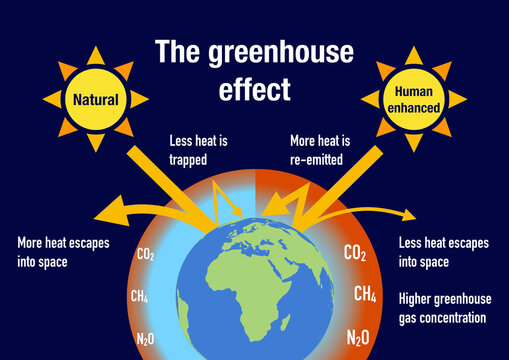
\includegraphics[width=\linewidth]{images/fig1.jpg}
	\caption{An illustration demonstrating the greenhouse effect, a natural phenomenon essential for life on Earth. Source: Adobe Stock.}
	\label{fig:Greenhouse Effect Illustration}
\end{figure}

\begin{figure}[H]
	\centering
	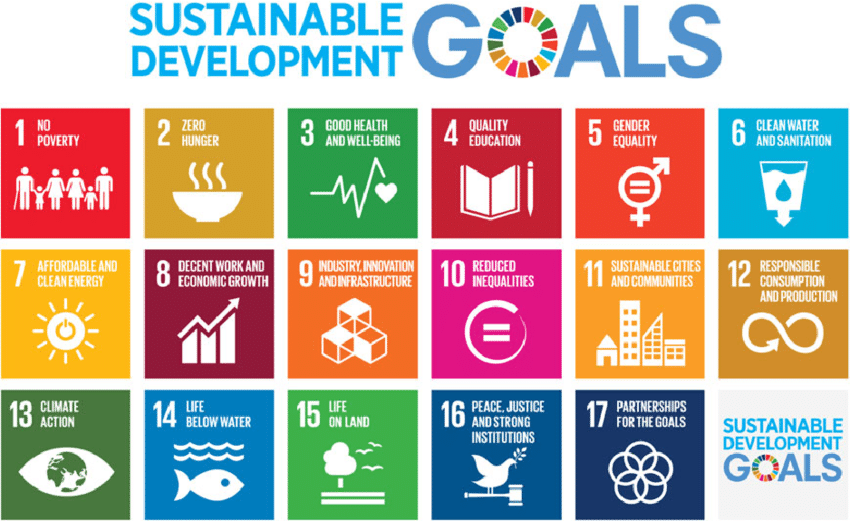
\includegraphics[width=\linewidth]{images/fig2.png}
	\caption{Graphic representation of the 17 Sustainable Development Goals set by the United Nations in 2015, focusing on various global challenges including environmental sustainability.}
	\label{fig:Sustainable Development Goals (SDG)}
\end{figure}

\begin{figure}[H]
	\centering
	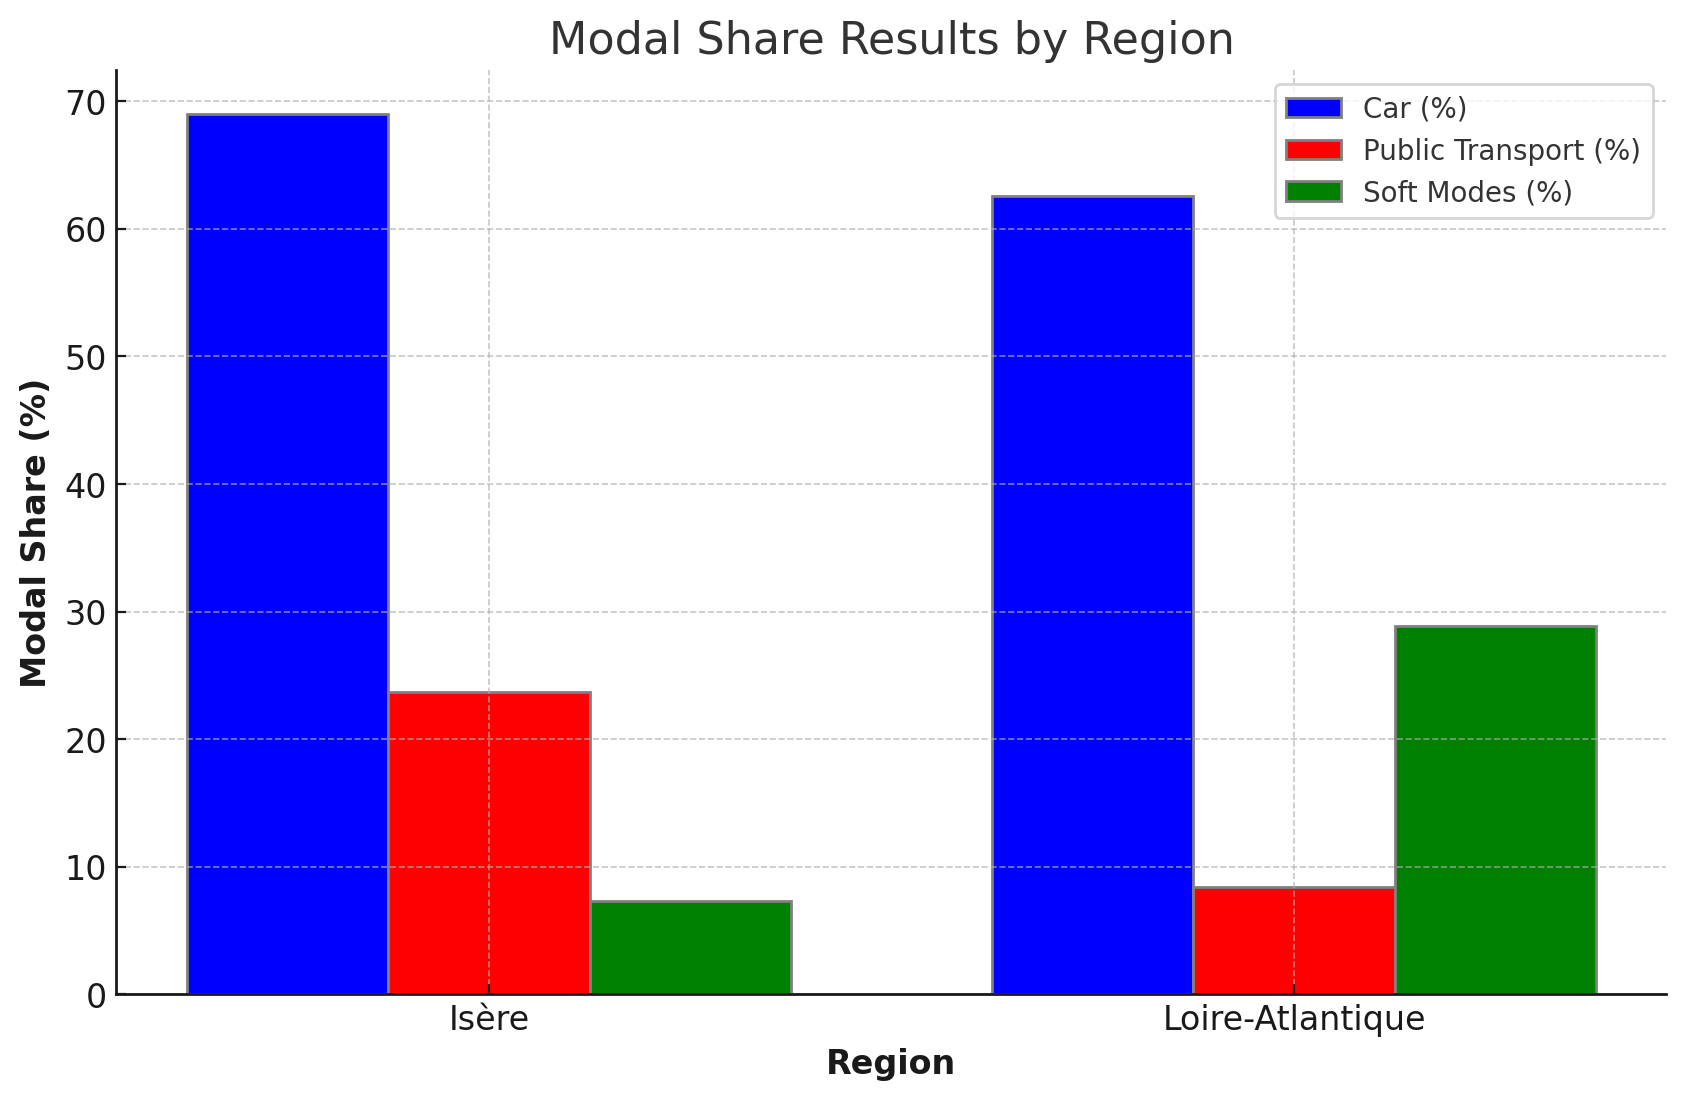
\includegraphics[width=\linewidth]{images/fig3.jpg}
	\caption{modal share results for the regions Isère and Loire-Atlantique. The graph shows the percentage distribution for different modes of transportation - car, public transport (pt), and soft modes - in each region. }
	\label{fig:modal_shared_results}
\end{figure}

\begin{figure}[H]
	\centering
	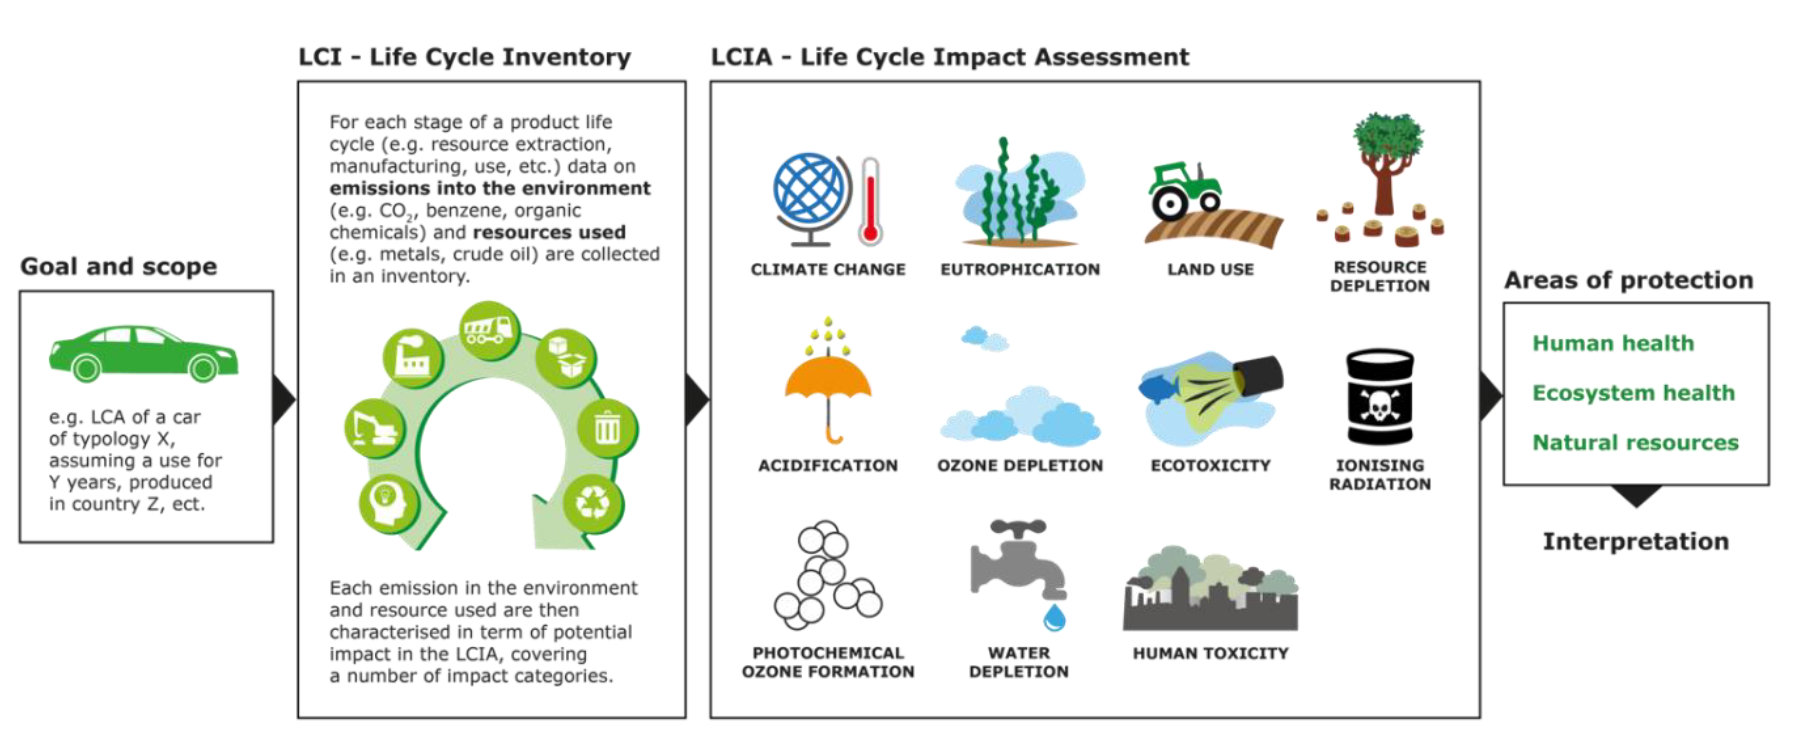
\includegraphics[width=\linewidth]{images/fig4.png}
	\caption{A cimage depicting the  indicators used in Life Cycle Assessment (LCA) for evaluating the environmental impact of cars Source: "Europeen Platform on Lifecycle Assesment"}
	\label{fig:Life Cycle Assessment (LCA) Categories}
\end{figure}

%plagiarism section - mandatory - do not remove, do not modify the content
\section*{Plagiarism statement}
\emph{This section is mandatory without modifications.}

I declare that I am aware of the following facts:
\begin{itemize}
	\item I understand that in the following statement the term "person" represents a human or \textbf{\textcolor{red}{ANY AUTOMATIC GENERATION SYTEM}}.
	\item As a student at the University of Luxembourg I must respect the rules of intellectual honesty, in particular not to resort to plagiarism, fraud or any other method that is illegal or contrary to scientific integrity.
	\item My report will be checked for plagiarism and if the plagiarism check is positive, an internal procedure will be started by my tutor. I am advised to request a pre-check by my tutor to avoid any issue.
	\item As declared in the assessment procedure of the University of Luxembourg, plagiarism is committed whenever the source of information used in an assignment, research report, paper or otherwise published/circulated piece of work is not properly acknowledged. In other words, plagiarism is the passing off as one’s own the words, ideas or work of another person, without attribution to the author. The omission of such proper acknowledgement amounts to claiming authorship for the work of another person. Plagiarism is committed regardless of the language of the original work used. Plagiarism can be deliberate or accidental.
	      Instances of plagiarism include, but are not limited to:
	      \begin{enumerate}
		      \item Not putting quotation marks around a quote from another person’s work
		      \item Pretending to paraphrase while in fact quoting
		      \item Citing incorrectly or incompletely
		      \item Failing to cite the source of a quoted or paraphrased work
		      \item Copying/reproducing sections of another person’s work without acknowledging the source
		      \item Paraphrasing another person’s work without acknowledging the source
		      \item Having another person write/author a work for oneself and submitting/publishing it (with permission, with or without compensation) in one’s own name (‘ghost-writing’)
		      \item Using another person’s unpublished work without attribution and permission (‘stealing’)
		      \item Presenting a piece of work as one’s own that contains a high proportion of quoted/copied or paraphrased text (images, graphs, etc.), even if adequately referenced
	      \end{enumerate}
	      Auto- or self-plagiarism, that is the reproduction of (portions of a) text previously written by the author without citing that text, i.e. passing previously authored text as new, may be regarded as fraud if deemed sufficiently severe.
\end{itemize}

\cleardoublepage
%% end-of-plagiarism section


\end{document}
